\section{Auswertung}

\subsection{Charakteristik des Geiger-Müllerzählrohrs}

Die gemessenen Daten zur Charakteristik des Geiger-Müllerzählrohrs sind in der Tabelle \ref{tab:ogemessdaten}
angegeben. Dabei ist die Zählrate %wie in .. erwähnt
gemäß der Poisson-Statistik verteilt, somit lässt sich der Fehler auf die Zählrate gemäß $\sqrt{N}$
bestimmen.

Zunächst sollen die Messpunkte mit einem Fehlerbalken in ein Diagramm eingezeichnet werden und anschließend soll entlang des Plateau-Bereiches
eine lineare Ausgleichsgerade erstellt werden. Graphisch lässt sich der Plateau-Bereich, also der Bereich in der die Zählrate kaum zunimmt bei ansteigender angelegten Spannung, grob
als Intervall von $\SI{370}{\volt}$ bis $\SI{630}{\volt}$ festlegen. Durch dieses Intervall kan nun eine lineare Ausgleichsgerade mit folgendem Ansatz gewählt werden.

\begin{equation}
y = a \cdot x + b
\end{equation}
wobei $a$ die Steigung der Geraden und $b$ der $y$-Achsenabschnitt ist.
Durch einen linearen Fit lassen sich die Parameter bestimmen zu

\begin{align}
a = \SI{1.138(241)}{\per\volt\per{60}\second}
\end{align}

\begin{figure}[h]
  \centering
  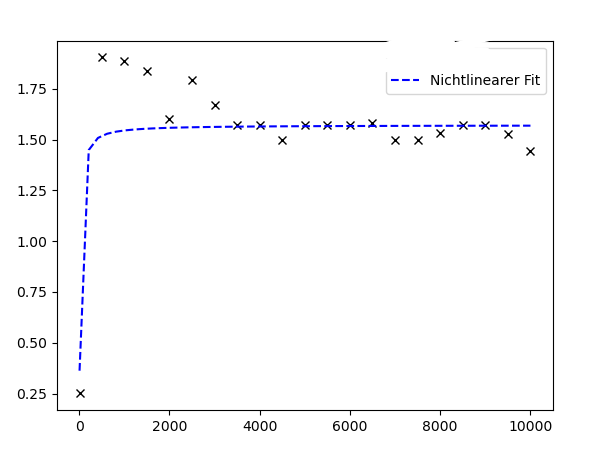
\includegraphics[width=\textwidth]{build/plot1.pdf}
  \caption{Messdaten und Fehlerbalken der Geiger-Müller Charakteristik}
  \label{fig:plot1}
\end{figure}